\chapter[TDTB+UJ]%
{Time Dependent Tight Binding+UJ}
\label{ch:one}
%
 \chapterquote{Le savant n'\'etudie pas la nature parce que cela est utile; \\
\indent il l'\'etudie parce qu'il y prend plaisir, \\ 
\indent et il y prend plaisir parce qu'elle est belle.}%
{by Henri Poincar\'e}
%
\section{Introduction}
\par{Tight binding is an approach to the quantum mechanical many particle problem particularly valuable in cases
where exact analytic solutions are not available (i.e. almost always) and other numerical approaches
like CI, DFT or GW are too time-consuming.}
\par{Tight binding methods lie between the very accurate and very expensive,
\emph{ab initio} methods, and the fast but limited, empirical methods. The
speed of the tight binding methods compared with the \emph{ab initio} is two
or three order of magnitude faster. Gaining speed we loose from the
transferability of the model, but in tight binding we retain the quantum
nature of the bonding. The tight binding methods are the ideal candidates, at
this time, for large size atomistic simulation. For an overview see e.g. \citep{Finnis03,Goringe97b}.}
\par{The relation between tight binding and density functional theory was
  investigated by \citep{Sutton88,Foulkes89,Frauenheim00}. In short, they
  proved that the tight binding models can be derived from DFT.}
\par{Different approximations made to full DFT total energy functional give us
different tight binding models. A common feature of all tight binding models
is the minimum basis set, that is taking into account  one $s$ orbital,
$3p$-orbitals, $5d$-orbitals
$\{\ket{s},\ket{p_x},\ket{p_y},\ket{p_x},\ket{d_{xy}},\ket{d_{yz}},\ket{d_{zx}},$
$\ket{d_{x^2-y^2}},\ket{d_{3z^2-r^2}}\}$
per atom. Principal quantum numbers do not have any meaning. The main
approximations that would define a tight binding model are: ignoring three
centre integrals, parametrise two centre integrals, ignore inter-site Coulomb,
assume orthogonality of orbitals, ignore charge transfer, a.s.o.}
\par{Usually a general tight binding model starts with the assumption that the
total energy can be written as}
\be
E=\sum_{i=1}^{N}\epsilon_i+\frac{1}{2}\sum_{i,j,i\neq j}U(R_{ij})
\ee
where $\epsilon_i$'s are the eigenvalues of a Schr{\"o}dinger-like equation
\be
\label{eigenschro}
H\ket{\psi_i}=\epsilon_i\ket{\psi_i}
\ee
$U(R_{ij})$ with $R_{ij}=|\vec{R_j}-\vec{R_i}|$ is a short-range pairwise
potential between the atoms $i$ and $j$.
\par{Eq. \gref{eigenschro} is solved in a minimal basis set of atomic like
localised functions $\{\phi_i\}$ which leads to the well known secular equation}
\be
|\underline{H}-\epsilon \underline{S}|=0
\ee
with matrices $\underline{H}$ and {\underline{S}} defined by
\be
H_{ij}=\bra{\phi_i}H\ket{\phi_j}\quad\quad S_{ij}=\Braket{\phi_i|\phi_j}
\ee
\par{Commonly we call $H_{ij}$ hopping integrals and $S_{ij}$ overlap
integrals. Another common feature is to consider $H_{ij}$, extending only to
first or second neighbours, as parameters taken from experiment or other
calculations. $\underline{S}=\underline{I}$ gives us what we call orthogonal
models.}
\par{Another important step is the use of two centre parametrisation of
Slater-Koster which gives us a fixed number of fundamental hopping integrals
(at least 4 for $sp$-systems - originally denoted as $ss\sigma$, $sp\sigma$,
$pp\sigma$, $pp\pi$). These parameters are interatomic
distances dependent. There is no absolute parametrisation for the interatomic distance
dependence, an exponential or an inverse power law being often used.}
\par{Our aim is to create a time dependent tight binding model which would help us to study
photoelectron transfer (PET) in sensor molecules \citep{deSilva01b}.}
\section[GSP scheme]{Goodwin-Skinner-Pettifor based scheme}
\par{Goodwin-Skinner-Pettifor (GSP) scheme was suggested in \citep{Goodwin89} and improved by Xu \emph{et al.}\citep{Xu92}. A recent improvement is added by Pettifor
\citep{Mrovec04}. The model that we use is based on Xu's implementation of
GSP scheme with two major differences which will be pointed when they would
appear. The total energy is given by}
\be
E=2\text{Tr}[\rho H]+\sum_{i}F\biggl(\sum_{j,i\neq j}\phi(R_{ij})\biggr)-2T_ek_B(\text{Tr}\rho\ln{\rho}+\text{Tr}(1-\rho)\ln{(1-\rho)})
\ee
where $i$, $j$ represents the atoms, $F(x)$ the embedded function for the
repulsive energy, $\phi(R_{ij})$ is the pair repulsive term between atom $i$
and $j$. Last term gives the ``temperature'' dependence of the model. In fact
is a trick used in order to improve the SCF models and to improve molecular dynamics. It represents the product $T_eS$ where
$T_e$ is ``the electronic temperature'' and $S$ is the entropy of a fermionic
gas. This is one of the improvements to the model.
\be
F(x)=\sum_{i=1}^{4}A_ix^i
\ee
with $A_i$'s parameters taken from \citep{Xu92}.
\be
\label{GSPscale}
\begin{split}
h_{\alpha}(r)=&V_{\alpha}\biggl(\frac{r_0}{r}\biggr)^n\exp{\biggl\{n\biggl[-\biggl(\frac{r}{r_c}\biggr)^{n_c}+\biggl(\frac{r_0}{r_c}\biggr)^{n_c}\biggr]\biggr\}}\\
\phi(r)=&\phi_0\biggl(\frac{d_0}{r}\biggr)^m\exp{\biggl\{m\biggl[-\biggl(\frac{r}{d_c}\biggr)^{m_c}+\biggl(\frac{d_0}{d_c}\biggr)^{m_c}\biggr]\biggr\}}
\end{split}
\ee
with $\alpha=ss\sigma,sp\sigma, ...$. $V_{\alpha}$ represents fundamental
hopping integral and $h_{\alpha}$ times angular factor given by Slater-Koster
parametrisation gives the inter site elements of the Hamiltonian. $r_0$
represents the first neighbour distance (bond length at equilibrium in our
case) all the rest quantities from \gref{GSPscale} are parameters to be
fit. $r_c$ is taken to lie somewhere in between first and second neighbours.
\par{Another set of parameters is represented by on-site energies
$\epsilon_{\alpha}$ ($\alpha=s,p,d, ...$)}
\be
\epsilon_{\alpha}^{i}=\bra{\alpha^i}H\ket{\alpha^i}
\ee
\par{To ensure energy conservation to $h_{\alpha}$ and $\phi$ tails are added. They
join the function at $r_1$ and are zero at $r_{cut}$. A simple polynomial form
is implemented such as to have continuous function and derivatives (first and
second) at $r_1$ and a zero function and derivatives (first and second) at
$r_{cut}$. This is the second difference from Xu's model. The tail function is}
\be
t(r)=(r-r_{cut})^3(10c+5br+3ar^2+5br_{cut}+4arr_{cut}+3ar_{cut}^2)/60
\ee
where $a,b,c$ are determined by the restrictions from definition of the
tail. Theirs values are
\be
\begin{split}
a=&\frac{10}{(r_1-r_{cut})^5}(12A-6Br_1+Cr_1^2+6Br_{cut}-2Cr_1r_{cut}+Cr_{cut}^2)\\
b=&-\frac{4}{(r_1-r_{cut})^5}(45Ar_1-21Br_1^2+3Cr_1^3+15Ar_{cut}+12Br_1r_{cut}-4Cr_1^2r_{cut}+9Br_{cut}^2\\&-Cr_1r_{cut}^2+2Cr_{cut}^3)\\
c=&-\frac{1}{(r_1-r_{cut})^5}(-60Ar_1^2+24Br_1^3-3Cr_1^4-60Ar_1r_{cut}+12Br_1^2r_{cut}-36Br_1r_{cut}^2\\&+8Cr_1^2r_{cut}^2-4Cr_1r_{cut}^3-Cr_{cut}^4)
\end{split}
\ee
with $A=f(r_1)$, $B=f^{\prime}(r_1)$, $C=f^{\prime\prime}(r_1)$
\par{This model was implemented in TDTB+UJ and used in all the
calculation presented in this thesis. Figures \gref{ssg} and \gref{spg}
show the radial part of hopping integrals $ss\sigma$ and $sp\sigma$ with a
tail added at $ r_1=1.5 \angstrom $ and a cut-off $ r_{cut}=1.9 \angstrom $, the rest of
parameters are taken from Table \gref{tablenh3} first SSA column and represent
fitted parameters for $N-H$ bond in our GSP-like model.}
\begin{figure}[!htb]
\begin{minipage}[!htb]{7.9cm}
\begin{center}
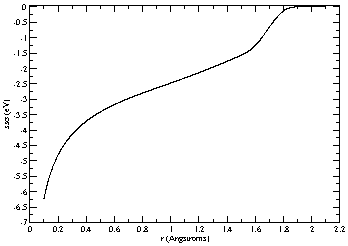
\includegraphics[width=7cm]{figures/ssg}
\end{center}
\caption{$ss\sigma$ radial dependence}
\label{ssg}
\end{minipage}
%\end{figure}
%
%\begin{figure}[!htb]
\begin{minipage}[!htb]{7.9cm}
\begin{center}
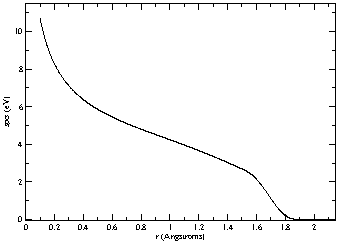
\includegraphics[width=7cm]{figures/spg}
\end{center}
\caption{$sp\sigma$ radial dependence}
\label{spg}
\end{minipage}
\end{figure}

\section{Introduction}
\par{The hamiltonian in second quantisation including electron-electron interaction term}
\begin{equation}
H=\sum_{i,\sigma}\epsilon_ia_{i\sigma}^{\dag}a_{i\sigma}+\sum_{i\neq j,\sigma}t_{ij}a_{i\sigma}^{\dag}a_{j\sigma}+\frac{1}{2}\sum_{ijkl\sigma \sigma{\prime}}
V_{ijkl}a_{i\sigma}^{\dag}a_{j\sigma\prime}^{\dag}a_{k\sigma\prime}a_{l\sigma}
\end{equation}
\par{$\sigma$ index stays for spin}
\par{first two terms are "normal" tight-binding terms}
\par{last term is the electron-electron interaction term.}
\par{Expanding the field operators in single particle eigenfunction we get}
\begin{equation}
\begin{split}
V_{ijkl}&=\int\phi_{i}^{*}(\bm{r})\phi_{l}(\bm{r})W(rr\prime)\phi_{j}^{*}(\bm{r^\prime})\phi_{k}(\bm{r^\prime})\td\bm{r}\td\bm{r^\prime}\\
&=\bra{ij}W\ket{lk}
\end{split}
\end{equation}
where $W(rr^\prime)=\frac{1}{4\pi\epsilon_0}\frac{e^2}{|\bm{r}-\bm{r^\prime}|}$.
\par{Electron-electron interaction from the point of view of field theory is: two particles in states $(l\sigma,k\sigma^\prime)$ interact and as a result two particles 
in the states $(i\sigma,j\sigma^\prime)$ emerge. Because of the nature of the hamiltonian, non-relativistic, the spin is conserved (no spin flip is described).}
\par{In tight-binding usually we ignore all the interactions described by such schemes.}
\par{Two type of such integrals are important for us direct and exchange Coulomb integrals.}
direct Coulomb integrals
\begin{equation}
\label{udef}
V_{ijji}=\int\phi_{i}^{*}(\bm{r})\phi_{i}(\bm{r})W(rr\prime)\phi_{j}^{*}(\bm{r^\prime})\phi_{j}(\bm{r^\prime})\td\bm{r}\td\bm{r^\prime}=U_{ij}
\end{equation}
$U_{ii}$ is the interaction energy associated with putting an elctron of spin up, let's say, into an orbital where there is already an electron with spin down.\\
exchange Coulomb integrals
\begin{equation}
V_{ijij}=\int\phi_{i}^{*}(\bm{r})\phi_{j}(\bm{r})W(rr\prime)\phi_{j}^{*}(\bm{r^\prime})\phi_{i}(\bm{r^\prime})\td\bm{r}\td\bm{r^\prime}=J_{ij}
\end{equation}
exchange energy only affects like spin electrons.
\par{Using the definition of $U$ from \gref{udef} we get a value of order $20eV$ which 
disagrees with experimental results. This come from the fact that the basis set is incomplete.
The incompletness of the basis set exclude any virtual transitions to these states.}
\par{+U formalism describes correctly the discontinuity in the potential as the occputaion number is changed (???Janak's theorem???).}
\section{The model}
\par{Assumptions:}
\begin{itemize}
\item{Not all electrons are correlated. These are separated out from the others identified by the orbitals they occupy or region of space or both.}
\item{When replacing an expectation value it is assumed that correlation exists only between electrons whose orbitals are on the same atom. }
\item{Only electrons with the same $n$within an atom are correlated}
\item {We use the \textit{mean field approximation} -- the two electron operator is expressed in term of a one electron operator acting alone but in the average field of the other}
\end{itemize}
\par{So, the expectation value of electron-electron interaction operator becomes}
\begin{equation}
\begin{split}
\frac{1}{2}&\sum_{ijkl\sigma\sigma^\prime}V_{ijkl}\langle a_{i\sigma}^{\dag}a_{j\sigma^\prime}^{\dag}a_{k\sigma^\prime}a_{l\sigma}\rangle
\cong \frac{1}{2}\sum_{ijkl\sigma\sigma^\prime}V_{ijkl}(\langle a_{i\sigma}^{\dag}a_{l\sigma} \rangle \langle a_{j\sigma^\prime}^{\dag}a_{k\sigma^\prime} \rangle -
\langle a_{i\sigma}^{\dag}a_{k\sigma^\prime}\rangle \langle a_{j\sigma^\prime}^{\dag}a_{l\sigma} \rangle )\\
&=\frac{1}{2}\sum_{ijkl\sigma\sigma^\prime}V_{ijkl}(n_{il}^{\sigma\sigma}n_{jk}^{\sigma^\prime\sigma^\prime}-
n_{ik}^{\sigma\sigma^\prime}n_{jl}^{\sigma^\prime\sigma})
\end{split}
\end{equation}
$n_{ij}^{\sigma\sigma^\prime}$ = generalised occupation numbers. (density matrix with non zero off-diagonal elements)\\
\par{Each index $ijkl$ stands for a $ \lbrace \bm{R}nlm \rbrace $ set, but having in mind our assumptions we realise
that $l,m$ are the only one which differs. We replace ${ijkl} \rightarrow {L_1L_2L_3L_4}$ with $L_i \rightarrow \lbrace l_im_i \rbrace$ and we get}
rewrite from here
\begin{equation*}
\begin{split}
E^U&=\frac{1}{2}\sum_{\{m_i\}\sigma\sigma^\prime}V_{m_1m_2m_3m_4}
(n_{m_1m_4}^{\sigma\sigma}n_{m_2m_3}^{\sigma^\prime\sigma^\prime}-
n_{m_1m_3}^{\sigma\sigma^\prime}n_{m_2m_4}^{\sigma^\prime\sigma})\\
&=\frac{1}{2}\sum_{\{m_i\}\sigma\sigma^\prime}V_{m_1m_2m_3m_4}
n_{m_1m_4}^{\sigma}n_{m_2m_3}^{\sigma^\prime}-\frac{1}{2}\sum_{\{m_i\}\sigma}V_{m_1m_2m_3m_4}
n_{m_1m_3}^{\sigma}n_{m_2m_4}^{\sigma}\\
&=\frac{1}{2}\sum_{\{m_i\}\sigma}V_{m_1m_2m_3m_4}n_{m_1m_4}^{\sigma}n_{m_2m_3}^{-\sigma}\\&-
\frac{1}{2}\sum_{\{m_i\}\sigma}V_{m_1m_2m_3m_4}
(n_{m_1m_3}^{\sigma}n_{m_2m_4}^{\sigma}-n_{m_1m_4}^{\sigma}n_{m_2m_3}^{\sigma})
\end{split}
\end{equation*}
\begin{equation}
\label{Eu}
\begin{split}
E^U=&\frac{1}{2}\sum_{\{m_i\}\sigma}V_{m_1m_2m_3m_4}n_{m_1m_4}^{\sigma}n_{m_2m_3}^{-\sigma}\\+&
\frac{1}{2}\sum_{\{m_i\}\sigma}(V_{m_1m_2m_3m_4}-V_{m_1m_2m_4m_3})
n_{m_1m_4}^{\sigma}n_{m_2m_3}^{\sigma}
\end{split}
\end{equation}
%
\par{The interaction potential associated with $E^U$ is given by}
\begin{equation*}
\p{E^U}{n_{mm^\prime}^{\sigma^\prime}}
\end{equation*}
%
\par{For simplicity we will compute it in two steps}
%
\begin{equation}
\begin{split}
V^{(1)}&=\frac{1}{2}\p{}{n_{mm^\prime}^{\sigma^\prime}}\sum_{\{m_i\}\sigma}V_{m_1m_2m_3m_4}n_{m_1m_4}^{\sigma}n_{m_2m_3}^{-\sigma}\\
&=\frac{1}{2}\sum_{\{m_i\}\sigma}V_{m_1m_2m_3m_4}(n_{m_2m_3}^{-\sigma}\delta_{m_1m}\delta_{m_4m^\prime}\delta_{\sigma\sigma^\prime}
+n_{m_1m_4}^{\sigma}\delta_{m_2m}\delta_{m_3m^\prime}\delta_{-\sigma\sigma^\prime})\\
&=\frac{1}{2}\sum_{m_2m_3}V_{mm_2m_3m^{\prime}}n_{m_2m_3}^{-\sigma^{\prime}}
+\frac{1}{2}\sum_{m_1m_4}V_{m_1mm^{\prime}m_4}n_{m_1m_4}^{-\sigma^{\prime}}\\
&=\sum_{m_1m_2}V_{mm_1m_2m^{\prime}}n_{m_1m_2}^{-\sigma^{\prime}}
\end{split}
\end{equation}
where for the last line we used $V_{m_1m_2m_3m_4}=V_{m_2m_1m_4m_3}$ and renamed the summation index.\\
\begin{equation}
\begin{split}
V^{(2)}&=\frac{1}{2}\p{}{n_{mm^\prime}^{\sigma^\prime}}\sum_{\{m_i\}\sigma}(V_{m_1m_2m_3m_4}-V_{m_1m_2m_4m_3})
n_{m_1m_4}^{\sigma}n_{m_2m_3}^{\sigma}\\
&=\sum_{m_1m_2}(V_{mm_1m_2m^{\prime}}-V_{mm_1m^{\prime}m_2})n_{m_1m_2}^{\sigma^\prime}
\end{split}
\end{equation}
So finally we get
\begin{equation}
V_{m_1m_2}^{\sigma}=\p{E^U}{n_{m_1m_2}^{\sigma}}=\sum_{m_3m_4}(V_{m_1m_3m_4m_2}
n_{m_3m_4}^{-\sigma}+(V_{m_1m_3m_4m_2}-V_{m_1m_3m_2m_4})n_{m_3m_4}^{\sigma})
\end{equation}
%
\par{Assuming real atomic-like orbitals $V$ becomes}
\begin{equation}
V_{n_1L_1n_2L_2n_3L_3n_4L_4}=\sum_{k=0}^{\infty}R^k(n_1l_1n_2l_2n_3l_3n_4l_4)A^k(L_1L_2L_3L_4)
\end{equation}
with
\begin{equation*}
A^k(L_1L_2L_3L_4)=\frac{4\pi}{2k+1}\sum_{p=-k}^{k}\mc{G}_{l_1m_1l_4m_4}^{kp}\mc{G}_{l_2m_2l_3m_3}^{kp}
\end{equation*}
but in our hypothesis we have
\begin{equation*}
l_1=l_2=l_3=l_4=l\qquad n_1=n_2=n_3=n_4=n
\end{equation*}
so 
\begin{equation*}
R^{k}(nlnlnlnl)=F^k(l,l)\text{ - Slater's Integrals}
\end{equation*}
\begin{equation}
V_{m_1m_2m_3m_4}=\sum_{k=0}^{2l}\frac{4\pi}{2k+1}F^k(l,l)\sum_{p=-k}^{k}\mc{G}_{lm_1lm_4}^{kp}\mc{G}_{lm_2lm_3}^{kp}
\end{equation}
\par{for the last relation we used the selection rules for Gaunt coefficients to get the sum limits for $k$.
$k$ must be also even.}
%
\section{+U for second order theory}
\par{We start by simply rewritting the density in the form $n=n^0+\delta n$, wehere $n^0$ is the reference density.
Now \gref{Eu} becomes}
\begin{equation}
\begin{split}
E^U&=\frac{1}{2}\sum_{\{m_i\}\sigma}V_{m_1m_2m_3m_4}(n_{m_1m_4}^{\sigma, 0}+\delta n_{m_1m_4}^{\sigma})(n_{m_2m_3}^{-\sigma,0}+\delta n_{m_2m_3}^{-\sigma})\\&+
\frac{1}{2}\sum_{\{m_i\}\sigma}(V_{m_1m_2m_3m_4}-V_{m_1m_2m_4m_3})
(n_{m_1m_4}^{\sigma,0}+\delta n_{m_1m_4}^{\sigma})(n_{m_2m_3}^{\sigma,0}+\delta n_{m_2m_3}^{\sigma})
\end{split}
\end{equation}
or
\begin{equation}
\label{eu2}
\begin{split}
E^U&=\frac{1}{2}\sum_{\{m_i\}\sigma}V_{m_1m_2m_3m_4}( n_{m_1m_4}^{\sigma, 0}n_{m_2m_3}^{-\sigma,0}+n_{m_1m_4}^{\sigma, 0}\delta n_{m_2m_3}^{-\sigma}
+ n_{m_2m_3}^{-\sigma,0}\delta n_{m_1m_4}^{\sigma}\\+& \delta n_{m_2m_3}^{-\sigma}\delta n_{m_1m_4}^{\sigma})+
\frac{1}{2}\sum_{\{m_i\}\sigma}(V_{m_1m_2m_3m_4}-V_{m_1m_2m_4m_3})
(n_{m_1m_4}^{\sigma, 0}n_{m_2m_3}^{\sigma,0}+n_{m_1m_4}^{\sigma, 0}\delta n_{m_2m_3}^{\sigma}
\\+& n_{m_2m_3}^{\sigma,0}\delta n_{m_1m_4}^{\sigma}+ \delta n_{m_2m_3}^{\sigma}\delta n_{m_1m_4}^{\sigma})
\end{split}
\end{equation}
\par{Now the potential associated with $E^U$ becomes}

\begin{equation}
\label{hamU}
\begin{split}
\mc{V}_{m_1m_2}^{\sigma}=\p{E^U}{\delta n_{m_1m_2}^{\sigma}}=&\sum_{m_3m_4}(V_{m_1m_3m_4m_2}
n_{m_3m_4}^{-\sigma,0}+(V_{m_1m_3m_4m_2}-V_{m_1m_3m_2m_4})n_{m_3m_4}^{\sigma,0})\\
+&\sum_{m_3m_4}(V_{m_1m_3m_4m_2}
\delta n_{m_3m_4}^{-\sigma}+(V_{m_1m_3m_4m_2}-V_{m_1m_3m_2m_4})\delta n_{m_3m_4}^{\sigma})
\end{split}
\end{equation}
%
\par{Now from the point of view of the second order theory the first term in \gref{hamU} should be added to $H^{in}$.
Second term represents the matrix element of the hamiltonian 
associated with $E_2$. The terms which contain only products of $n^0$ in \gref{eu2} can be regarded as a reference energy. No forces arise from \gref{eu2}. So, we have}
%
\begin{equation}
\begin{split}
E_{2}^{U}&=\frac{1}{2}\sum_{\{m_i\}\sigma}\left [V_{m_1m_2m_3m_4}\delta n_{m_2m_3}^{-\sigma}\delta n_{m_1m_4}^{\sigma}\right. \\&\left.+
(V_{m_1m_2m_3m_4}-V_{m_1m_2m_4m_3})
\delta n_{m_2m_3}^{\sigma}\delta n_{m_1m_4}^{\sigma}\right]\\
H^{U,\sigma}_{2m_1m_2}&=\sum_{m_3m_4}(V_{m_1m_3m_4m_2}
\delta n_{m_3m_4}^{-\sigma}+(V_{m_1m_3m_4m_2}-V_{m_1m_3m_2m_4})\delta n_{m_3m_4}^{\sigma})\\
H^{in(U), \sigma}_{m_1m_2}&=\sum_{m_3m_4}(V_{m_1m_3m_4m_2}
n_{m_3m_4}^{-\sigma,0}+(V_{m_1m_3m_4m_2}-V_{m_1m_3m_2m_4})n_{m_3m_4}^{\sigma,0})\\
E^{U}_{ref}&=\frac{1}{2}\sum_{\{m_i\}\sigma}\left[V_{m_1m_2m_3m_4}n_{m_1m_4}^{\sigma, 0}n_{m_2m_3}^{-\sigma,0}\right. \\ &\left.+(V_{m_1m_2m_3m_4}-V_{m_1m_2m_4m_3})
n_{m_1m_4}^{\sigma, 0}n_{m_2m_3}^{\sigma,0}\right]
\end{split}
\end{equation}
%
\section{Outline}
+U formalism
\par{1. adds electron-electron interaction}
\par{2. restricted to the onsite terms and oritals with the same $l$}

\section{On currents}
\par{to cite Tchavdar's papers on the subject. notations this should be collected and used a the begining of the chapter.}
\par{$\Set{\Ket{I\mu}}$ - basis set}
\par{$\Ket{I\mu}$ an orbital centred on atom $I$}
\par{$\Ket{\Psi}=\sum_{I,\mu}c_{I\mu}\Ket{I\mu}$ a general electronic state, where $c_{I\mu}$ are the expansion coefficients}
\par{We assume that we have an orthogonal basis set}
\be{equation}
\braket{I\mu | J_nu}=\delta_{IJ}\delta_{\mu\nu}
\ee
\par{The Hamiltonian is}
\be
\Hamiltonian=\sum_{I\mu J\nu}\Braket{I\mu | \Hamiltonian_{I\mu J\nu} | J\nu}
\ee
\be
\Hamiltonian_{I\mu J\nu}=\Braket{I\mu | \Hamiltonian | J\mu}
\ee
\be
\Hamiltonian\Ket{\Psi(t)}=i\hbar \Ket{\dot{\Psi}(t)}
\ee
\be
\Hamiltonian\Ket{\Psi}=E\Ket{\psi} 
\ee
\par{$E$ is the energy eigenvalue}
\par{Let us define the projection operator}
\be
\mc{P}_{I}=\sum_{\mu} \Ket{I\mu}\Bra{I\mu}
\ee
\par{it represents the electron occupancy of atomic site $I$. It satisfies the following closure relation}
\be
\sum_{I}\mc{P}_{I}=\bm{I}
\ee
\be
\bm{P}_{I}=\Braket{\Psi(t) | \mc{P}_{I} |\Psi(t)}
\ee
\par{Let us calculate $\dot{\bm{P}}_{I}(t)$}
\be
\begin{split}
\dot{\bm{P}}_{I}(t)&=\de{}{t}\left[\Braket{\Psi(t) | \mc{P}_{I} |\Psi(t)}\right]\\
 &=\Braket{\dot{\Psi}(t) | \mc{P}_{I} |\Psi(t)}+\Braket{\Psi(t) | \mc{P}_{I} |\dot{\Psi}(t)}
\end{split}
\ee
\par{using time dependent Schr\"{o}dinger equation}
\be
\begin{split}
\Ket{\dot{\Psi}(t)}=&\frac{1}{i\hbar}\Hamiltonian\Ket{\Psi(t)}\\
\Bra{\dot{\Psi}(t)}=&-\frac{1}{i\hbar}\Bra{\Psi(t)}\Hamiltonian
\end{split}
\ee
\par{we get}
\be
\begin{split}
\dot{\bm{P}}_{I}(t)=&-\frac{1}{i\hbar}\Braket{\Psi(t) | \mc{HP}_{I} | \Psi(t)}+\frac{1}{i\hbar}\Braket{\Psi(t) | \mc{P}_{I}\Hamiltonian |\Psi(t)}\\
 =&\frac{1}{i\hbar}\Braket{\Psi(t) | \Commutator{\mc{P}_{I}}{\Hamiltonian} | \Psi(t)}
\end{split}
\ee
\par{Now we can define}
\be
\mc{J}_{I}=\frac{1}{i\hbar}\Commutator{\mc{P}_{I}}{\Hamiltonian}
\ee
\be
\begin{split}
\mc{J}_{I}=&\frac{1}{i\hbar}\left( \mc{P}_{I}\Hamiltonian - \Hamiltonian\mc{P}_{I}  \right)\\
=&\frac{1}{i\hbar}\left( \mc{P}_{I}\Hamiltonian\bm{I} - \bm{I}\Hamiltonian\mc{P}_{I}  \right)\\
=&\sum_{J\neq I}\left( \mc{P}_{I}\Hamiltonian\mc{P}_{J} - \mc{P}_{J}\Hamiltonian\mc{P}_{I} \right)
\end{split}
\ee
\par{we define}
\be
\mc{J}_{J\mapsto I}=\frac{1}{i\hbar}\left(\mc{P}_{I}\Hamiltonian{H}\mc{P}_{J} - \mc{P}_{J}\Hamiltonian\mc{P}_{I} \right)
\ee
\par{it represents the electronic particle current from site $J$ to site $I$, it may be thought as a bond current. This expression is derived under the orthonormal basis assumption.}
\be
\begin{split}
\mc{J}_{J\mapsto I}=&\frac{1}{i\hbar}\left(\sum_{\mu,\nu}\Ket{I\mu}\Bra{I\mu}\Hamiltonian\Ket{J\nu}\Bra{J\nu}-\sum_{\mu,\nu}\Ket{J\nu}\Bra{J\nu}\Hamiltonian\Ket{I\mu}\Bra{I\mu}\right)\\
=&\frac{1}{i\hbar}\left(\sum_{\mu,\nu}\Ket{I\mu}\Hamiltonian_{I\mu J\nu}\Bra{J\nu}-\sum_{\mu,\nu}\Ket{J\nu}\Hamiltonian_{J\nu I\mu}\Bra{I\mu}\right)
\end{split}
\ee
\par{and now we can compute easily the matrix elements of the bond current operator.}
\be
\begin{split}
\mc{J}_{J\mapsto I}\Ket{K\kappa}=&\frac{1}{i\hbar}\left(\sum_{\mu,\nu}\Ket{I\mu}\Hamiltonian_{I\mu J\nu}\Braket{J\nu | K\kappa}-\sum_{\mu,\nu}\Ket{J\nu}\Hamiltonian_{J\nu I\mu}\Braket{I\mu | K\kappa}\right)\\
=&\frac{1}{i\hbar}\left(\sum_{\mu}\Ket{I\mu}\Hamiltonian_{I\mu J\kappa}\delta_{JK}-\sum_{\nu}\Ket{J\nu}\Hamiltonian_{J\nu I\kappa}\delta_{IK}\right)
\end{split}
\ee
%
\be
\begin{split}
\Braket{L\lambda | \mc{J}_{J\mapsto I} | K\kappa}=\mc{J}_{J\mapsto I}^{L\lambda K\kappa}=\frac{1}{i\hbar}\left(\Hamiltonian_{I\lambda J\kappa}\delta_{JK}\delta_{IL}-\Hamiltonian{H}_{J\lambda I\kappa}\delta_{IK}\delta_{JL}\right)
\end{split}
\ee
\par{the average electron particle current from $J$ to $I$ is}
\be
\begin{split}
\tm{J}_{J\mapsto I}=&\Trace\left( {\mc{J}_{J\mapsto I}\rho}\right)=\sum_{A\alpha B\beta}\mc{J}_{J\mapsto I}^{A\alpha B\beta}\rho_{A\alpha B\beta}\\
=&\frac{1}{i\hbar}\sum_{A\alpha B\beta}\left( \Hamiltonian_{I\alpha J\beta}\delta_{IA}\delta_{JB}-\Hamiltonian_{J\alpha I\beta}\delta_{IB}\delta_{JA}\right)\rho{B\beta A\alpha}
 \end{split}
\ee
\par{using the fact that \Hamiltonian is real and the hermicity of $\rho$}
\be
\begin{split}
 \tm{J}_{J\mapsto I}=&\frac{1}{i\hbar}\sum_{\alpha \beta}\Hamiltonian_{I\alpha J\beta}\left(\rho_{J\beta I\alpha}-\rho_{I\alpha J\beta}\right)=\frac{1}{i\hbar}\sum_{\alpha \beta}\Hamiltonian_{I\alpha J\beta}\left(\rho_{J\beta I\alpha}-\rho_{J\beta I\alpha}^{*}\right)\\ \\
=&\frac{2}{\hbar}\sum_{\alpha \beta}\Hamiltonian_{I\alpha J\beta}\bm{Im}\rho_{J\beta I\alpha}
\end{split}
\ee
\par{and we define the bond current}
\be
\tm{J}_{J\mapsto I}=\frac{2e}{\hbar}\sum_{\alpha \beta}\Hamiltonian_{I\alpha J\beta}\bm{Im}\rho_{J\beta I\alpha}
\ee
\par{We can find a continuity equation for our current and density}
\be
\begin{split}
\bm{P}_I=&\Trace\left( \mc{P}\hat{\rho}\right)\\
\dot{\bm{P}}_I=&\Trace\left( \mc{P}\dot{\hat{\rho}}\right)	
\end{split}
\ee
\par{We recall the equation for $\dot{\hat{\rho}}$}
\be
\dot{\hat{\rho}}=\frac{1}{i\hbar}\Commutator{\Hamiltonian}{\hat{\rho}}-\Gamma\left(\hat{\rho}-\hat{\rho_0}\right)
\ee
\be
\dot{\bm{P}}_{I}=\Trace\left(\mc{P}_{I}\frac{1}{i\hbar}\Commutator{\Hamiltonian}{\hat{\rho}}\right)-\Gamma \Trace \left( \mc{P}_{I}\left(\hat{\rho}-\hat{\rho_0}\right)\right)
\ee
\be
\begin{split}
 \Trace&\left( \mc{P}_{I}\Commutator{\Hamiltonian}{\hat{\rho}}\right)=-\Trace\left( \mc{P}_{I}\Commutator{\hat{\rho}}{\Hamiltonian}\right)\\
 =&-\Trace\left(\Commutator{\mc{P}_I\hat{\rho}}{\Hamiltonian}-\Commutator{\mc{P}_I}{\Hamiltonian}\hat{\rho}\right)\\
 =&\Trace \left(\Commutator{\mc{P}_{I}}{\Hamiltonian}\hat{\rho}\right)
\end{split}
\ee
\par{Where we used the well known commutators properties}
\be
\begin{split}
 \Commutator{\bm{AB}}{\bm{C}}&=\bm{A}\Commutator{\bm{B}}{\bm{C}}+\Commutator{\bm{A}}{\bm{C}}\bm{B}\\
 \Trace&\left(\Commutator{\bm{A}}{\bm{B}}\right)=0
\end{split}
\ee
\be
\dot{\bm{P}}_{I}=\Trace \left(\frac{1}{i\hbar}\Commutator{\mc{P}_{I}}{\Hamiltonian}\hat{\rho}\right)-\Gamma(\bm{P}_{I}-\bm{P}_{0})
\ee
\be
\dot{\rho}_{II}=\sum_{J \neq I}\tm{J}_{J\mapsto I}-\Gamma\Delta\rho_{II}
\ee
\section{Magnetic field of bond currents}
\par{We wan to compute the magnetic field created by the bond current in a ring molecule, see figure \ref{fig:MagneticField}. For simplicity, but without the loss of generality, we consider the molecule laying the x-y plane. The problem can be broken in two parts. Part one compute the magnetic field due to a finite length wire and part two add all the contributions.}
\par{Part one can be formulated as:}
\par{\emph{Compute the magnetic field generated by a wire (AB) of finite length, $L$, carrying a constant current $I_0$. The wire is parallel with the y-axis and the current flows in the direction of the y-axis. The distance between the y-axis and the wire is $R$.}}
\begin{figure}[!ht]
\begin{center}
\scalebox{1.2}{\input{bfield.tex}}
\caption{Geometry of the finite length wire}
\label{fig:MagneticField}
\end{center}
\end{figure}
\par{The current in the wire can be written as}
\be
\bm{j}(\bm{r},t)=I_0\delta(z)\delta(x-R)\Theta(y-a)\Theta(a+L-y)\versor{y}
\label{eq:current}
\ee
\par{where $\delta$ represents the Dirac function and $\Theta$ the Heaviside step function.}
\par{We can compute very simple, using the retarted potentials, the vector potential $\bm{A}(\bm{r},t)$}
\be
\bm{A}(\bm{r},t)=\frac{\mu_0}{4\pi}\int\td^3\bm{r'}\td{t'}\cfrac{\delta\left(t'-t+\cfrac{|\bm{r}-\bm{r'}|}{c}\right)}{|\bm{r}-\bm{r'}|}\bm{j}(\bm{r},t)
\ee
\par{there is no time dependence in the current so the time integral is straight-forward}
\be
\bm{A}(\bm{r},t)=\frac{\mu_0}{4\pi}\int\td^3\bm{r'}\cfrac{1}{|\bm{r}-\bm{r'}|}\bm{j}(\bm{r},t)
\ee
\par{with}
\ben
\begin{split}
 \bm{r}=&x\versor{x}+y\versor{y}+z\versor{z}\\
\bm{r'}=&R\versor{x}+y'\versor{y}\\
|\bm{r}-\bm{r'}|=&\sqrt{(x-R)^2+(y-y')^2+z^2}=l\\
d^2=&(x-R)^2+z^2
\end{split}
\een
\par{and equation \gref{eq:current} $\bm{A}$ becomes}
\be
\bm{A}(\bm{r},t)=\frac{\mu_0I_0}{4\pi}\versor{y}\int\td x'\td y'\td z'\cfrac{\delta(z')\delta(x'-R)\Theta(y'-a)\Theta(a+L-y')}{l}
\ee
\be
\bm{A}(\bm{r},t)=\frac{\mu_0I_0}{4\pi}\versor{y}\int_{a}^{a+L}\frac{\td y'}{l}
\ee
\par{now we can compute very simple the magnetic field $\bm{B}$}
\be
\bm{B}=\nabla\times\bm{A}=
\left|\begin{array}{ccc}
       \versor{x} & \versor{y} & \versor{z}  \\
       \p{}{x} & \p{}{y} & \p{}{z} \\
        0 & \bm{A}_y & 0
      \end{array}
 \right| = -\p{\bm{A}_y}{z}\versor{x}+\p{\bm{A}_y}{x}\versor{z}
\ee
\be
\begin{split}
 \p{}{z}\frac{1}{l}=&\p{}{z}\frac{1}{\sqrt{(x-R)^2+(y-y')^2+z^2}}=-\cfrac{z}{\left[(x-R)^2+(y-y')^2+z^2\right]^{3/2}}\\
 \p{}{x}\frac{1}{l}=&\p{}{x}\frac{1}{\sqrt{(x-R)^2+(y-y')^2+z^2}}=-\cfrac{x-R}{\left[(x-R)^2+(y-y')^2+z^2\right]^{3/2}}
\end{split}
\ee
\par{so \bm{B} becomes}
\be
\bm{B}=\frac{\mu_0I_0}{4\pi}\int_{a}^{a+L}\frac{\td y'}{\left(d^2+(y-y')^2\right)^{3/2}}\left(z\versor{x}-(x-R)\versor{z}\right)
\ee
\par{the integral is}
\be
\int\frac{\td y'}{\left(d^2+(y-y')^2\right)^{3/2}}=\frac{1}{d^2}\frac{y'-y}{\sqrt{d^2+(y-y')^2}}+\mc{C}
\ee
\par{so}
\be
\bm{B}=\frac{\mu_0I_0}{4\pi d^2}\left[\frac{a+L-y}{\sqrt{d^2+(a+L-y)^2}}-\frac{a-y}{\sqrt{d^2+(a-y)^2}}\right]\left(z\versor{x}-(x-R)\versor{z}\right)
\ee
